\section{Programação Paralela e Vetorial em OpenMP}\label{sec:openmp}

Os modelos de programação paralela são divididos em modelos de memória compartilha e de memória distribuída. Exemplos de modelos de programação em memória compartilhada são OpenMP (\emph{Open Multi-Processing})~\cite{openmp,chapman2008using}, Cilk~\cite{reinders2012overview,robison2013composable} e CUDA (\emph{Compute Unified Device Architecture})~\cite{cook2012cuda,kirk2016programming}. Nesse ambiente, a programação é feita utilizando \textit{threads}. A decomposição utilizada é na sua maioria a decomposição do domínio ou a funcional, com diferentes granularidades. No caso dos modelos de memória distribuída, o MPI (\emph{Message Passing Interface})~\cite{gropp1999using,pitt2017introduction} é um dos mais utilizados. Nesse modelo, a programação é feita utilizando processos distribuídos. A decomposição utilizada é do domínio, buscando a maior granularidade possível. 

Neste capítulo, optou-se por utilizar OpenMP, focando em memória compartilhada. OpenMP é uma API (\emph{Application Programming Interface}) de programação paralela portável para arquiteturas de memória compartilhada. OpenMP surgiu da dificuldade no desenvolvimento de programas paralelos em arquiteturas de memória compartilhada, além da ausência de APIs padronizadas para tais arquiteturas. A interface proporciona diretivas que possibilitam expressar paralelismo de dados, em trechos de código e laço, e paralelismo de tarefas, introduzido em sua versão 3.0~\cite{AyguadeCoptyDuranEtAl2009}. Sua API é constituída de diretivas de compilação, métodos de biblioteca e variáveis de ambiente. Em sua versão 4.0~\cite{martineau2016evaluating}, OpenMP inclui suporte para dependências de dados em tarefas e suporte a aceleradores~\cite{openmp}. No momento da escrita desse minicurso, OpenMP estava em sua versão 5.0~\cite{de2018ongoing}.

Alguns fatores limitam o desempenho dos códigos paralelos. O primeiro fator é o próprio código sequencial. Existem partes do código que são inerentemente sequenciais como, por exemplo, iniciar e terminar a computação. Essas partes do código não são aceleráveis. Outro fator é a concorrência, ou seja, o número de tarefas pode ser escasso ou de difícil definição. Por exemplo, pode-se ter um processador com 40 \textit{cores}, mas a aplicação possuir apenas 10 iterações de laço que podem ser divididas. Outros dois pontos que limitam muito o desempenho das aplicações são a comunicação e a sincronização. Existe sempre um custo associado à troca de informação e enquanto as tarefas sincronizam essa informação, elas não contribuem para a computação. 
A partilha de dados entre as várias tarefas pode levar a problemas de contenção no acesso à memória e enquanto as tarefas ficam à espera da sincronização elas não podem computar nada. Por fim, o balanceamento de carga é muito importante, pois ter os processadores maioritariamente ocupados durante toda a execução é decisivo para o desempenho global do sistema.

\subsection{Programando com OpenMP}

A API OpenMP é composta basicamente por diretivas de compilação e métodos da biblioteca. As diretivas são anotações no código e os métodos OpenMP dependem da compilação com a biblioteca. As diretivas de compilação, \emph{pragmas} em linguagem C/C++, do OpenMP começam com \texttt{\#pragma omp} e são seguidos por construções e cláusulas que se aplicam a um bloco estruturado. As construções descrevem seções paralelas, dividem dados ou tarefas entre \textit{threads} e controlam sincronização. Por sua vez, as cláusulas modificam ou especificam aspectos das construções.

O primeiro exemplo é um \emph{Olá Mundo}. A Figura~\ref{fig:omp:hello} ilustra o primeiro exemplo em OpenMP. A construção \texttt{parallel} indica um bloco de execução paralela, ou seja, faz com que o bloco estruturado especificado entre as linhas \ref{fig:omp:hello:bloc1} e \ref{fig:omp:hello:bloc2} seja executado uma vez para cada \textit{thread} criada. O ambiente OpenMP irá alocar um determinado número de \textit{threads}, e todas elas executarão as linhas de comando contidas dentro do \texttt{parallel}. O número de \textit{threads} varia, sendo responsabilidade do programador garantir que o resultado esperado seja atingido independentemente do número de \emph{threads}. A compilação de tal programa com o compilador \texttt{gcc} necessita da opção \texttt{-fopenmp}, como no exemplo abaixo:

\begin{lstlisting}[frame=none, numbers=none]
@\textcolor{mygreen}{\$ gcc -fopenmp -o hello hello.c}@
\end{lstlisting}

\begin{figure}[!htb]
\centering
\begin{lstlisting}
#include <stdio.h>
#include <omp.h>

int main(){
   int myid, nthreads;
   
   @\textcolor{mygreen}{\#pragma omp parallel private(myid)}@
@\label{fig:omp:hello:bloc1}@   @\textcolor{mygreen}{\{}@ 
      myid = omp_get_thread_num();
      nthreads = omp_get_num_threads();

      printf("Hello world. I am thread %d of %d\n",
                myid, nthreads);
@\label{fig:omp:hello:bloc2}@   @\textcolor{mygreen}{\}}@
   return 0;
}
\end{lstlisting}
\caption{Exemplo de um \emph{Hello world} em OpenMP.}
\label{fig:omp:hello}
\end{figure}

A execução ocorre da mesma forma que qualquer outro programa em um terminal. Se nenhum argumento é especificado, o programa utilizará todos os \textit{cores} disponíveis no processador. Em nosso exemplo, assumindo que a máquina possui um processador de dois \textit{cores}, a execução será:

\begin{lstlisting}[frame=none, numbers=none]
@\textcolor{mygreen}{\$ ./hello}@
0 of 2 - hello world!
1 of 2 - hello world!
\end{lstlisting}

Na linha de comando, pode-se alterar o número de \textit{threads} com a variável de ambiente \verb+OMP_NUM_THREADS+. Por exemplo, com 4 \textit{threads}:
\begin{lstlisting}[frame=none, numbers=none]
@\textcolor{mygreen}{\$ OMP\_NUM\_THREADS=4 ./hello}@
0 of 4 - hello world!
1 of 4 - hello world!
2 of 4 - hello world!
3 of 4 - hello world!
\end{lstlisting}

\subsection{Modelo de Execução}
\label{sec:omp:modelo}

O paralelismo em OpenMP é chamado \emph{fork/join}, ou seja, o programa inicia com uma \textit{thread}, a \textit{thread} inicial. Ao encontrar uma construção \texttt{parallel}, o programa cria ou bifurca (\emph{fork}) um grupo de \textit{threads} que executam um bloco estruturado de código. Essas \textit{threads} são então unidas (\emph{join}) ao final do bloco.

A Figura~\ref{fig:omp:model} mostra um exemplo de execução OpenMP com três regiões paralelas. A \textit{thread} inicial, que encontra a construção \texttt{parallel}, é chamada de \textit{thread} \textbf{master}. Ela é responsável por criar um grupo de \textit{threads} que executará o bloco paralelo. As regiões sequenciais são aquelas fora da construção \texttt{parallel} e são executadas pela \textit{thread} master. Por outro lado, as regiões paralelas executam nos \textit{cores} disponíveis e podem variar o número de \emph{threads} no decorrer da execução. Nesse exemplo (Figura~\ref{fig:omp:model}) existem três regiões paralelas com quatro, seis e três \emph{threads}, respectivamente.

\begin{figure}[!htb]
\centering
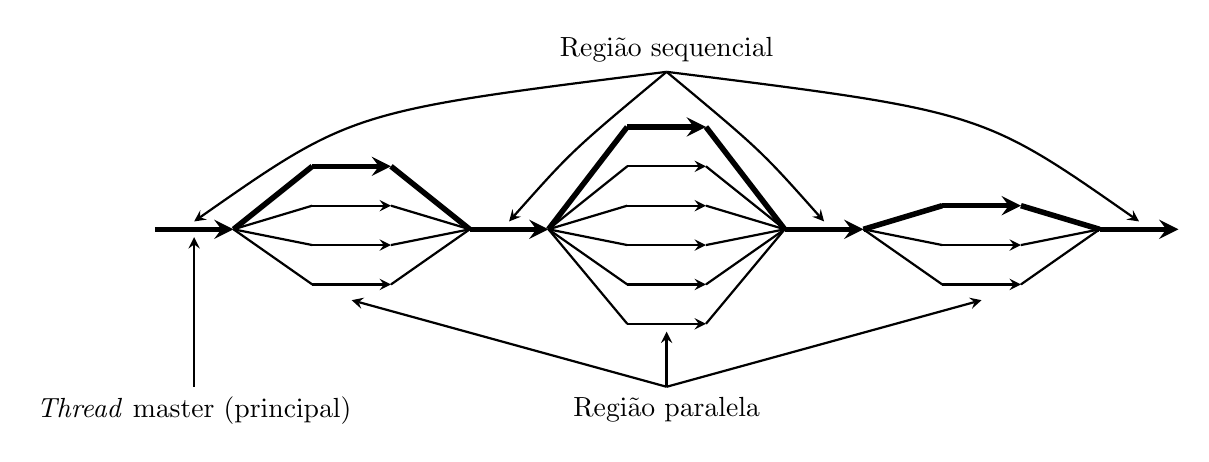
\begin{tikzpicture}[style=thick, >=stealth]%[line width=2pt]
\begin{scope}[line width=2pt]
  \draw[->] (0,0) -- (1,0);
  %
  \draw (1,0) -- (2,0.8);
  \draw[->] (2,0.8) -- (3,0.8);
  \draw (3,0.8) -- (4,0);
\end{scope}
%
\draw (1,0) -- (2,0.3);
\draw[->] (2,0.3) -- (3,0.3);
\draw (3,0.3) -- (4,0);
%
\draw (1,0) -- (2,-0.2);
\draw[->] (2,-0.2) -- (3,-0.2);
\draw (3,-0.2) -- (4,0);
%
\draw (1,0) -- (2,-0.7);
\draw[->] (2,-0.7) -- (3,-0.7);
\draw (3,-0.7) -- (4,0);
%
\begin{scope}[line width=2pt]
  \draw[->] (4,0) -- (5,0);
  %
  \draw (5,0) -- (6,1.3);
  \draw[->] (6,1.3) -- (7,1.3);
  \draw (7,1.3) -- (8,0);
\end{scope}
%
\draw (5,0) -- (6,0.8);
\draw[->] (6,0.8) -- (7,0.8);
\draw (7,0.8) -- (8,0);
%
\draw (5,0) -- (6,0.3);
\draw[->] (6,0.3) -- (7,0.3);
\draw (7,0.3) -- (8,0);
%
\draw (5,0) -- (6,-0.2);
\draw[->] (6,-0.2) -- (7,-0.2);
\draw (7,-0.2) -- (8,0);
%
\draw (5,0) -- (6,-0.7);
\draw[->] (6,-0.7) -- (7,-0.7);
\draw (7,-0.7) -- (8,0);
%
\draw (5,0) -- (6,-1.2);
\draw[->] (6,-1.2) -- (7,-1.2);
\draw (7,-1.2) -- (8,0);
%
\begin{scope}[line width=2pt]
  \draw[->] (8,0) -- (9,0);
  %
%  \draw (9,0) -- (10,0.8);
%  \draw[->] (10,0.8) -- (11,0.8);
%  \draw (11,0.8) -- (12,0);
\draw (9,0) -- (10,0.3);
\draw[->] (10,0.3) -- (11,0.3);
\draw (11,0.3) -- (12,0);
%
\end{scope}
%
\draw (9,0) -- (10,-0.2);
\draw[->] (10,-0.2) -- (11,-0.2);
\draw (11,-0.2) -- (12,0);
%
\draw (9,0) -- (10,-0.7);
\draw[->] (10,-0.7) -- (11,-0.7);
\draw (11,-0.7) -- (12,0);
%
\draw[->,line width=2pt] (12,0) -- (13,0);
%
\draw[<-] (2.5,-0.9) -- (6.5,-2) node[below] {Região paralela};
\draw[<-] (6.5,-1.3) -- (6.5,-2);
\draw[<-] (10.5,-0.9) -- (6.5,-2);
%
\draw[<-] (0.5,-0.1) -- (0.5,-2) node[below] {\textit{Thread} master (principal)};
%
\draw[<-] (4.5,0.1) ..  controls(5.3,1) .. (6.5,2) node[above] {Região sequencial};
\draw[<-] (0.5,0.1) .. controls(2.5,1.5) .. (6.5,2);
\draw[<-] (8.5,0.1) .. controls(7.7,1) .. (6.5,2);
\draw[<-] (12.5,0.1) .. controls(10.5,1.5) .. (6.5,2);
%
\end{tikzpicture}
\caption{Modelo de execução \emph{fork/join} do OpenMP.}
\label{fig:omp:model}
\end{figure}

A execução dentro de um bloco \texttt{parallel} é SPMD (\textit{single program multiple data}), ou seja, as \textit{threads} do grupo executam o mesmo código. A execução em SPMD é amplamente utilizada em alto desempenho e principalmente conhecida por seu uso em programas MPI. Cada \textit{thread} possui um identificador como veremos a seguir.

\subsection{Métodos de Biblioteca}
\label{sec:omp:biblio}

Os métodos da biblioteca OpenMP atuam para modificar e monitorar \textit{threads}, processos e a região paralela do programa. Elas são ligadas como funções externas em C. É necessário incluir a biblioteca no arquivo fonte do código ( com \texttt{\#include <omp.h>}). A seguir são listadas as principais funções de OpenMP:

\begin{description}
\item \verb+void omp_set_num_threads(int N)+

Modifica o número de \textit{threads} da próxima região paralela.
\item \verb+int omp_get_num_threads()+

Retorna o número de \emph{threads} ativas naquele momento da execução.
\item \verb+int omp_get_thread_num()+

Retorna o identificador da \emph{thread} atual, também conhecido como \emph{id}.
\end{description}

Um exemplo de uso dessas funções pode ser visto na Figura~\ref{fig:omp:hello}.

\subsection{Cláusulas de Dados}
\label{sec:omp:dados}

O OpenMP é uma API de programação paralela para memória compartilhada, então grande parte das variáveis em memória são compartilhadas. Porém, nem todas as varáveis podem ser compartilhadas. Por exemplo, variáveis da pilha de funções e automáticas (de blocos de código) dentro de uma região paralela são privadas.

O OpenMP permite especificar e modificar o modo de acesso dentro de construções \texttt{parallel} por meio de cláusulas. As cláusulas para dados em OpenMP são:

\begin{description}
\item[private] - cria uma cópia local da memória para cada \textit{thread}. Não inicializa as cópias criadas e não mantém o valor após o fim da execução da região paralela.
\item[shared] - indica que a variável é compartilhada entre todas as \textit{threads}. Esse é o padrão quando nada é especificado.
\item[firstprivate] - cria uma cópia local da memória para cada \textit{thread}, e inicializa cada uma com o último valor fora da região paralela.
\item[lastprivate] - copia o valor da última iteração dentro da região paralela para a variável única após a região paralela.
\end{description}

\subsection{Laços Paralelos}
\label{sec:omp:loop}

Os laços paralelos são uma das principais construções do OpenMP devido a sua popularidade e ocorrência em aplicações paralelas. O laço paralelo distribui as iterações entre as \textit{threads} disponíveis, o que justifica a construção ser chamada \textbf{worksharing}.

A Figura~\ref{fig:omp:loop} mostra um exemplo de laço paralelo em OpenMP, onde a soma das posições do vetor \texttt{v} será dividido entre as \textit{threads} da região paralela. As construções \texttt{parallel} e \texttt{for} podem ser combinadas em uma única linha como em \texttt{\#pragma omp parallel for}, isso, caso exista apenas uma região \texttt{for} dentro da região paralela.

\begin{figure}[!htb]
\centering
\begin{lstlisting}[escapeinside={@}{@}]
long long int sum(int *v, long long int N){
   long long int i, sum_local, sum = 0;

   @\textcolor{mygreen}{\#pragma omp parallel private(i, sum\_local)}@
   @\textcolor{mygreen}{\{}@
     sum_local = 0;

     @\textcolor{mygreen}{\#pragma omp for}@
     for(i = 0; i < N; i++)
       sum_local += v[i];

     @\textcolor{mygreen}{\#pragma omp atomic}@
     sum += sum_local;
   @\textcolor{mygreen}{\}}@
   return sum;
}
\end{lstlisting}
\caption{Laço paralelo com OpenMP.}
\label{fig:omp:loop}
\end{figure}

\subsection{Exclusão Mútua}
\label{sec:omp:sync}

Uma pergunta que surge é como as \textit{threads} de programas paralelos interagem? Como foi visto, OpenMP é um modelo de memória compartilhada. Nesse sentido, as \textit{threads} comunicam-se através de variáveis compartilhadas. Ao longo da execução do programa, podem acontecer compartilhamentos não intencionais de dados causando condições de corrida. 
Uma condição de corrida ocorre quando a saída do programa muda caso as \textit{threads} sejam escalonadas de uma forma diferente. O problema existe quando duas ou mais \textit{threads} tentam alterar as mesmas posições de memória como na Tabela~\ref{tb:openmp:sum:race}. Nesta representação, deseja-se fazer a soma de todos elementos de um vetor, considerando que há 2 \textit{threads} e que todos os elementos do vetor são iguais a~1. Entre os tempos 1 e 4 tudo ocorre como esperado. Porém, nos tempos 5 e 6, as operações de ambas as \textit{threads} se sobrepõem, fazendo literalmente que uma das operações de soma seja perdida, causando um resultado errado.

\begin{table}[!htb]
\centering
\caption{Exemplo de execução do código de soma dos elementos de um vetor com o problema das condições de corrida.}
\label{tb:openmp:sum:race}
\begin{tabular}{@{}cll@{}}
  \toprule
  Tempo & Thread 0            & Thread 1         \\
  \midrule
  1    & Ler sum=0           &                  \\
  \midrule
  2    & Escrever sum=1      &                  \\
  \midrule
  3    &                     & Ler sum=1        \\
  \midrule
  4    &                     & Escrever sum=2   \\
  \midrule
  5    & Ler sum=2           & Ler sum=2        \\
  \midrule
  6    & Escrever sum=3      & Escrever sum=3   \\
  \bottomrule
\end{tabular}
\end{table}

Para resolver tal problema, utilizou-se a sincronização. A sincronização é necessária em programação paralela a fim de coordenar a execução e evitar condições de corrida. Em OpenMP pode-se encontrar diversas formas de sincronização desde controle de ordem de execução até regiões críticas. Vale a pena lembrar que a sincronização é cara e, por isso, tenta-se mudar a forma de acesso aos dados para minimizar a necessidade de sincronizações.

A sincronização assegura que uma ou mais \textit{threads} estão em um estado bem definido em um ponto conhecido da execução. As duas formas mais comuns de sincronização são a barreira e a exclusão mútua. Na barreira, cada \textit{thread} espera na barreira até a chegada de todas as demais. Já a exclusão mútua, define um bloco de código onde apenas uma \textit{thread} pode executar por vez. 

Para a barreira, utiliza-se a diretiva \texttt{barrier}. Para exclusão mútua, pode-se usar duas diretivas: \texttt{critical} e \texttt{atomic}. 
A diretiva \texttt{critical} especifica que o bloco de código é uma região crítica e apenas uma \textit{thread} por vez executa a região. A diretiva \texttt{atomic} tem o mesmo objetivo, entretanto, diferente da \texttt{critical} que é implementada em \textit{software}, a \texttt{atomic} é implementada em \textit{hardware} utilizando instruções especiais da arquitetura. 
A diretiva \texttt{atomic} é muito veloz em relação a \texttt{critical}, entretanto, ela só implementa um conjunto de operações específicas que incluem incrementos, atribuições e operações simples. A Figura~\ref{fig:omp:loop} mostra um exemplo de uso do \texttt{atomic}, onde um valor é acumulado. A acumulação é atômica e concorrente.

Além dessas diretivas, existem outras, como a \texttt{master}, que define uma região em que apenas a \textit{thread}~0 executa. Caso não seja necessário que a \textit{thread}~0 execute, mas apenas uma das \emph{threads}, pode ser utilizada a construção \texttt{single}. Outra diferença entre a diretiva \texttt{single} e a \texttt{master} é que a \texttt{single} adiciona uma barreira implícita após seu término. Isto é, apesar de apenas uma \textit{thread} executar o bloco \texttt{single}, todas as outras \textit{threads} ficam aguardando a execução finalizar para prosseguir. Caso não seja necessária a barreira, deve-se adicionar a diretiva \texttt{nowait} ao comando resultando em \texttt{\#pragma omp single nowait}.

\subsection{Redução}

Em algumas situações, as aplicações paralelas precisam reduzir ou acumular um certo valor de forma concorrente dentro de um laço. Essa situação é bem comum, e chama-se redução. O suporte a tal operação é fornecido pela maioria dos ambientes de programação paralela. Tal funcionalidade é suportada em OpenMP com a cláusula \texttt{reduction}. Basicamente, uma redução é a combinação de variáveis locais de uma \textit{thread} em uma variável única. 

Uma redução em OpenMP possui a sintaxe \verb+reduction (op : list)+, onde \texttt{op} é a operação e \texttt{list} é a lista de variáveis a serem acumuladas. Dentro de um bloco cada variável de \texttt{list} gera uma cópia local (por \textit{thread}) e é inicializada de acordo com a operação (ex.: \texttt{0} para a operação \texttt{+}). Atualizações por iteração acontecem localmente em cada \textit{thread} e, ao fim do bloco (\emph{join}), as cópias locais são reduzidas em um valor único e combinadas com o valor original. Note que as variáveis em \texttt{list} devem ser compartilhadas (\texttt{shared}) dentro da região paralela.

\begin{figure}[!htb]
\centering
\begin{lstlisting}[escapeinside={@}{@}]
long long int sum(int *v, long long int N){
   long long int i, sum = 0;

   @\textcolor{mygreen}{\#pragma omp parallel for private(i) reduction(+ : sum)}@
   for(i = 0; i < N; i++)
     sum += v[i];

   return sum;
}
\end{lstlisting}
\caption{Exemplo do cálculo de soma de vetor com redução em OpenMP.}
\label{fig:omp:reduction2}
\end{figure}

Na Figura~\ref{fig:omp:reduction2} o cálculo da soma de todos os elementos de um vetor \texttt{v} é utilizado como exemplo. Anteriormente calculou-se este resultado utilizando somas locais. O exemplo difere do anterior por conter a adição da construção \texttt{parallel for} com a operação de redução \texttt{+} para acumular os resultados na variável \verb+sum+. As operações suportadas pela redução são \texttt{+}, \texttt{-}, \texttt{*}, \texttt{min}, \texttt{max}, \verb+&+, \verb+|+, \verb+^+, \verb+&&+ e \verb+||+.

\subsection{Vetorização}

O paralelismo com execução vetorial ocorre de forma diferente do paralelismo em \textit{multicore}. Enquanto na execução normal cada instrução opera em apenas um dado, na instrução vetorial a mesma operação é executada em vários dados de forma independente~\cite{satish2012can}. Considerando o laço apresentado na Figura~\ref{fig:omp:simd}, que soma dois vetores e armazena o resultado em um terceiro, pode-se perceber que as iterações do laço são independentes. 
Supondo que há instruções para ler e escrever 8 operandos na memória, e somar 8 operandos, pode-se visualizar o mesmo laço sendo operado vetorialmente, operando 8 por unidade de tempo utilizando o \texttt{\#pragma omp simd}.

A lógica deste comando é semelhante ao \texttt{pragma omp for}, com a diferença que agora o paralelismo dá-se vetorialmente. Ele também aceita a cláusula \texttt{reduction}, sendo que, é responsabilidade do programador assegurar que as iterações são independentes.

Em relação ao exemplo, cada iteração do laço carrega 8 operandos a partir da posição~$i$ dos vetores $b$ e $c$, soma-se cada par \mbox{$(b[i], c[i])$} de forma independente, e depois o bloco de 8~operandos é escrito no vetor~$a$ a partir da posição~$i$. O número de operandos por unidade de tempo depende tanto do tamanho do dado quanto do tamanho da unidade vetorial do processador alvo.

\begin{figure}[!htb]
\centering
\begin{lstlisting}[escapeinside={@}{@}]
void sum(int *a, int *b, int *c, long long int N){
   long long int i;

   @\textcolor{mygreen}{\#pragma omp simd}@
   for(i = 0; i < N; i++)
     a[i] = b[i] + c[i]
}
\end{lstlisting}
\caption{Exemplo do cálculo de soma de dois vetores com SIMD.}
\label{fig:omp:simd}
\end{figure}

As instruções vetoriais já estão presentes há muitos anos em processadores x86. A cada nova geração, aumenta-se a quantidade de dados processados por instrução, bem como o número de instruções vetoriais disponíveis. É importante ressaltar que, para maior eficiência, os endereços acessados no laço em iterações sucessivas devem ser consecutivos.